\documentclass[a4paper]{article}

\usepackage{graphicx}
\usepackage[utf8]{inputenc}
\usepackage[colorlinks]{hyperref}
\usepackage{listings}

% OK? TEIL				SOLL	IST
% [x] Titel, Abstract	0.5		0.5
% [x] Introduction		1		0.7
% [x] Background		1.5		2
% [x] Related Work		1		2
% [x] Mapping			3		2.5
% [x] Implementierung	1		0.5
% [x] Example			2		2.5
% [x] Conclusion		1		1
%     Referenzen		1.5		1.2
%     Gesamt			12		12.5

\title{Mapping BPMN Diagrams to JIAC Agent Beans}
\author{Tobias K\"uster \and Petrus Setiawan Tan \and Axel He\ss{}ler}
\date{}

\bibliographystyle{abbrv}
\lstset{basicstyle=\scriptsize, tabsize=2}

\begin{document}

	\maketitle

	\begin{abstract}
		% Problem
		Different mappings from processes to agents have been proposed, but using
		restricted process models or targeting only single agents, none of them
		is very convincing.
		% Motivation
		This is a pity, since business processes have many notions in common with
		agents and would be well suited for modelling complex multi-agent systems.
		% Solution
		In this paper, we combine two of the existing approaches, namely WADE and
		the mapping from BPMN to JADL, to a mapping from BPMN to JIAC Agent Beans.
		% Contribution
		The resulting Agent Beans are well-structured and extensible, and at the
		same time account for nearly all of the expressiveness of BPMN.
	\end{abstract}

	%%%%%%%%%%%%%%%%%%%%%%%%%%%%%%%%%%%%%%%%%%%%%%%%%%%%%%%%%%%%%%%%%%%%%%%%%%%%%%%%
%%                                                                            %%
%%  INTRODUCTION                                                              %%
%%                                                                            %%
%%%%%%%%%%%%%%%%%%%%%%%%%%%%%%%%%%%%%%%%%%%%%%%%%%%%%%%%%%%%%%%%%%%%%%%%%%%%%%%%

% [x] Problem
% [x] Motivation
% [x] Solution
% [x] Contribution
% [x] Outline

\section{Introduction}
\label{sec:intro}

% Problem
In recent times, different approaches have been introduced, using business
process diagrams or related notations for modelling agents and multi-agent
systems~\cite{caire2008wade,kuester2010integrating}.  However, none of these
approaches is really compelling.  Often, very simple workflow models are used, or
if a more expressive process modelling notation, such as BPMN~\cite{omg2009bpmn}
is used, only a limited subset of the language is covered.  Further, usually only
single agents are targeted, while interactions between agents -- which could very
well be modelled using e.g. BPMN -- are not regarded.

% Motivation
This is a pity, since process diagrams -- particularly complex notations such as
the Business Process Modeling Notation (BPMN) -- share many concepts and abstractions
with multi-agent systems.  Besides the actual workflow, those notations can be
used for modelling several participants in a process, as well as their interactions
and communication, or their reactions to external events, centring much more on
the \emph{what} and less on the \emph{how}.  Thus, despite the shortcomings of
existing approaches, BPMN and related notations appear to be very well suited for
modelling agents and particularly multi-agent systems.

% Solution
In this paper we take a look at some of the existing approaches -- the WADE
extension to the JADE agent framework, and the mapping from BPMN to JIAC's
scripting language JADL -- and try to combine the strong sides of both into a new
approach.  The result is a mapping from BPMN to JIAC Agent Beans, following the
basic principles of WADE, but using a much more expressive process notation.

% Contribution
This way, JIAC Agent Beans, being the core components of the agents, can be
generated easily from BPMN processes.  The resulting Java classes are similarly
structured and extensible as the JADE classes of WADE, but reflect the whole BPMN
process, including communication between agents and event-handling, both as part
of the workflow and for triggering the process.


%%%%%%%%%%%%%%%%%%%%%%%%%%%%%%%%%%%%%%%%%%%%%%%%%%%%%%%%%%%%%%%%%%%%%%%%%%%%%%%%

% Outline
The remainder of this paper is structured as follows: In Section~\ref{sec:background}
we will give a short introduction to both, the BPMN process modelling language,
and the JIAC multi-agent framework.  Then, in Section~\ref{sec:related} we will
have a look at related work, most notably the WADE framework and the mapping from
BPMN to JADL.  Thereafter, we will describe in detail how BPMN processes can be
mapped to semantically equivalent JIAC Agent Beans (Section \ref{sec:mapping}),
and how the transformation has been implemented (Section~\ref{sec:impl}).
In Section~\ref{sec:example}, the mapping is illustrated using an example,
before we finally discuss our results in Section~\ref{sec:conclusion}.


	%%%%%%%%%%%%%%%%%%%%%%%%%%%%%%%%%%%%%%%%%%%%%%%%%%%%%%%%%%%%%%%%%%%%%%%%%%%%%%%%
%%                                                                            %%
%%  BACKGROUND                                                                %%
%%                                                                            %%
%%%%%%%%%%%%%%%%%%%%%%%%%%%%%%%%%%%%%%%%%%%%%%%%%%%%%%%%%%%%%%%%%%%%%%%%%%%%%%%%

% [x] Intro
% [x] BPMN
% [x] JIAC

\section{Background}
\label{sec:background}

% Mini-Intro
In the following, we will introduce the reader to the BPMN language and the JIAC
agent framework, being the domain an co-domain of the mapping proposed in this
paper.


%%%%%%%%%%%%%%%%%%%%%%%%%%%%%%%%%%%%%%%%%%%%%%%%%%%%%%%%%%%%%%%%%%%%%%%%%%%%%%%%

\subsection{BPMN}
\label{sec:bpmn}

% Standard, Einsatzgebiet, etc.
The Business Process Modeling Notation~\cite{omg2009bpmn} is a workflow notation
which can be used both as a description language for real-world processes, and as
a high-level modelling language for computer programs -- most prominently BPEL
processes.  It can be seen as a combination of UML's Activity Diagrams and Sequence
Diagrams, depicting both the actors' internal processes and their interactions.
An example diagram is shown in Figure~\ref{fig:example} in Section~\ref{sec:example}.

% 3 Levels of BPMN
BPMN diagrams can be understood at three levels of abstraction:

\begin{enumerate}
	\item The diagrams are made up of a few easily recognisable elements, i.e.\
	Events (circles), Activities (boxes) and Gateways (diamonds), connected by
	Sequence- and Message Flows and situated in one or more Pools.
	
	\item These basic elements are further distinguished using sets of marker
	icons, e.g.\ Message, Timer, and Error Events, or parallel and exclusive
	Gateways.
	
	\item Each element features a number of additional attributes, which are
	hidden from the diagram, but contain all the information that is necessary
	for automated code generation, e.g. properties and assignments.
\end{enumerate}

Consequently, the essence of a BPMN diagram is easily understood by all business
partners, including those who have great knowledge in their domain but little
understanding of programming and multi-agent systems.  At the same time, BPMN
diagrams provide enough information for the generation of executable programs.

% interessante Sprachfeatures: Rollen, Messaging, etc.
BPMN diagrams have a variety of notational elements, making them well suited for
the design of distributed systems in general and multi-agent systems in particular.
The process diagrams are subdivided into Pools, each representing one Participant
in the process.  Using Message Flows for communication between Pools, even complex
interaction protocols can be modelled clearly.  Further, the notation supports
features such as event- and error handling, compensation, transactions and
\emph{ad-hoc}-behaviour.

% Semantik nicht ganz klar, wird aber besser
While the semantics of some elements of BPMN -- particularly those not covered in
the official mapping from BPMN to BPEL~\cite[Appendix A]{omg2009bpmn} -- are not
very clearly defined, there is an increasing number of approaches describing the
semantics of BPMN using e.g.\ Petri nets~\cite{dijkman2008formal}, and version
2.0 of the specification makes things clearer, too.

% XXX wenn noetig, hier kuerzen

% Wieso nicht Petrinetze?
The reason why Petri nets are not used in the first place is that while Petri
nets have very clear semantics, and basically everything can be expressed as a
Petri net, some high-level constructs that are directly supported by BPMN would
result in huge, incomprehensible Petri nets.

% Positiver Schlusssatz
BPMN is neither the first process modelling notation, nor will it be the last.
However, given its high level of adoption in practical process modelling
\cite{recker2008bpmnmodeling} and its relatively detailed execution semantics,
it has proven to be a good choice for modelling distributed computing systems.


%%%%%%%%%%%%%%%%%%%%%%%%%%%%%%%%%%%%%%%%%%%%%%%%%%%%%%%%%%%%%%%%%%%%%%%%%%%%%%%%

\subsection{JIAC}
\label{sec:jiac}

% Intro JIAC und Features
JIAC V (Java Intelligent Agent Componentware, Version 5) is a Java-based
multi-agent development framework and runtime environment \cite{hirsch2009jiacv}.
Among others, JIAC features communication, tuple-space based memory, transparent
distribution of agents and services, and provides support for dynamic reconfiguration
in distributed environments, such as component exchange at runtime.  Individual
JIAC agents are situated within Agent Nodes, i.e. runtime containers, which also
provide support for strong migration.  The agents' behaviours and capabilities
are defined in a number of so-called \emph{Agent Beans}, which are controlled by
the agent's life cycle.

% Standard Agent Beans
One Agent Bean each JIAC agent is equipped with is the \emph{Communication Bean},
allowing agents to send and receive messages to and from other agents or groups
of agents (broadcasting to message channels).  The messages are not restricted to
FIPA messages but can have any serialisable data as payload.  Other commonly used
Agent Beans are the \emph{Rule Engine Bean}, integrating a Drools\footnote{JBoss
Drools: \url{http://www.jboss.org/drools/}} rule engine into the agent's memory,
and the \emph{Interpreter Bean}, providing an interpreter for the service-oriented
scripting language JADL++~\cite{hirsch2010programming}.

% Custom Beans
Besides these and other predefined Agent Beans, the programmer is free to add
more Beans to the agent.  Each Agent Bean can

\begin{itemize}
	\item implement a number of \emph{life-cycle} methods, which are executed when
	the agent changes its life-cycle state, such as initialized, or started,
	
	\item implement an \emph{execute}-method, which is called automatically at
	regular intervals once the agent is running,
	
	\item attach \emph{observers} to the agent's memory, being called e.g. each
	time the agent receives a message or a percept is updated, and
	
	\item contribute any number of \emph{action}-methods, which are exposed to the
	directory and can be invoked by other agents or other beans of the same agent.
\end{itemize}

% Schlusssatz, Verweis auf Manual
Using these four mechanisms, it is possible to define all of the agents' capabilities
and behaviours.  For details on programming JIAC Agent Beans, please refer to the
JIAC Programmers' Manual~\cite{jiacManual}.


	%%%%%%%%%%%%%%%%%%%%%%%%%%%%%%%%%%%%%%%%%%%%%%%%%%%%%%%%%%%%%%%%%%%%%%%%%%%%%%%%
%%                                                                            %%
%%  RELATED WORK                                                              %%
%%                                                                            %%
%%%%%%%%%%%%%%%%%%%%%%%%%%%%%%%%%%%%%%%%%%%%%%%%%%%%%%%%%%%%%%%%%%%%%%%%%%%%%%%%

% [x] Intro
% [x] BPMN -> BPEL
% [x] BPMN -> JADL
% [x] WADE
% [x] GO-BPMN

\section{Related Work}
\label{sec:related}

In the following we will discuss several works which are highly relevant to the
approach described in this paper: The original mapping from BPMN to BPEL, a
mapping from BPMN to JIAC's scripting language JADL, the WADE framework, mapping
workflows to JADE behaviours, and GO-BPMN, a combination of BPMN and goal hierarchies.


%%%%%%%%%%%%%%%%%%%%%%%%%%%%%%%%%%%%%%%%%%%%%%%%%%%%%%%%%%%%%%%%%%%%%%%%%%%%%%%%

\subsection{Mapping BPMN to BPEL}

One of the motivations for developing BPMN was to provide a standardised graphical
notation for \emph{BPEL}, the Business Process Executable Language.  Consequently,
a mapping from BPMN to BPEL is part of the BPMN specification~\cite[Appendix
A]{omg2009bpmn}, and a number of alternative or extended mappings have been
proposed by various other authors (see for example~\cite{ouyang2009business}).
% , making heavy use of BPEL event handlers).

In many aspects, the mapping is very straightforward, as it is evident that BPMN
was created with the mapping to BPEL in mind: Each Pool is mapped to a BPEL
process (which can be deployed as a Web service), and the several events and
activities within are mapped to the workflow of the process.  The process is made
up mostly of Web service calls, assignments and flow control, but can also contain
e.g. event handling based on timing and incoming messages.  Given a sufficiently
detailed BPMN diagram, the resulting BPEL process can be readily executable.

Still, there are enough elements in BPMN for which no mapping to BPEL is given,
i.e. BPMN is not just a visualization for BPEL but an individual language -- and
in fact more expressive than BPEL itself.  Amongst the elements which are not
mapped to BPEL are somewhat esoteric elements such as the \emph{ad-hoc} subprocess,
or the complex gateway, but also many kinds of events and tasks.


%%%%%%%%%%%%%%%%%%%%%%%%%%%%%%%%%%%%%%%%%%%%%%%%%%%%%%%%%%%%%%%%%%%%%%%%%%%%%%%%

\subsection{Mapping BPMN to JADL}

% erste Version des Mapping nach JADL gemacht, SOA+Agenten-Sprache
In prior work of mapping BPMN to JIAC agents, JIAC's service-oriented scripting
language \emph{JADL}~\cite{hirsch2010programming} was selected as the target of
the transformation.

% Behaviours werden in JADL beschrieben
Being conceptually close to BPEL, the mapping is similar, and the process can be
mapped very directly to different language elements of JADL -- for instance, like
BPEL, JADL has dedicated language elements for complex actions such as invoking
another service, or for sending and receiving messages, making the generated code
compact and easy to comprehend.  Similar to the mapping to BPEL, each Pool in the
BPMN process is mapped to a JADL service, and the service's input parameters and
result types are derived from the Pool's start- and end
events~\cite{kuester2010integrating}.

% Starter-Regeln mit Drools
Further, for each start event, a Drools rule is created, starting the respective
JADL service on the occurrence of the given event (e.g. an incoming message, or
a given time).

% Agenten-Konfiguration
Finally, for each Participant in the BPMN process, an XML-based agent configuration
file is created, setting up the individual agents, each equipped with an Interpreter
Bean and Rule Engine Bean, together with the generated JADL services and Drools
rules.  Alternatively, the JADL services created from the BPMN processes can be
deployed to a running JIAC agent, thus dynamically changing its behaviour.


%%%%%%%%%%%%%%%%%%%%%%%%%%%%%%%%%%%%%%%%%%%%%%%%%%%%%%%%%%%%%%%%%%%%%%%%%%%%%%%%

\subsection{WADE: Workflows for JADE}

% WADE: JADE + Workflows
A different approach, from which some of the concepts in this work have been
drawn, is \emph{WADE (Workflows and Agents Development Environment)}, which is
an extension to the JADE multi-agent framework~\cite{bellifemine1999jade}.
With WADE, certain aspects of the behaviour of a JADE agent can be modelled
using a simple workflow notation~\cite{caire2008wade,caire2010wade}, based on
which Java classes are generated.  The workflows basically consist of only two
elements: Activities and Transitions.

% generiert Java-Code, pro Aktivität ein Methodenrumpf, Workflow-Inheritance
Using the \emph{Wolf} tool~\cite{caire2008wolf}, JADE behaviour classes can be
generated from those workflow models.  In the generated Java classes, there is
a clear distinction between the workflow (the order of the activities, together
with conditions and guards, where required) and the several activities, each of
which is mapped to an individual Java method, which can either refer to existing
functionalities or be implemented by the developer.  Using this separation,
generated workflows can easily be altered or extended.

% Schlecht: sehr einfache Workflow-Notationen, nichts agentisches
However, the expressiveness of WADE is restricted by the simplistic workflow
model, which allows only the most basic workflows to be modelled.  While the
transitions can be annotated with guards (conditions), it seems impossible to
model parallel execution and synchronisation, let alone more advanced concepts
such as event handling or messaging.  In fact, each workflow diagram covers only
the behaviour of an isolated agent; to our knowledge, interactions between agents
can not be modelled.


%%%%%%%%%%%%%%%%%%%%%%%%%%%%%%%%%%%%%%%%%%%%%%%%%%%%%%%%%%%%%%%%%%%%%%%%%%%%%%%%

\subsection{GO-BPMN}
% XXX wenn noetig, hier kuerzen (Intro nicht vergessen)

% Worum es bei GO-BPMN geht: Zielhierarchien und Prozesse, Kritik der Autoren
In another approach, \emph{GO-BPMN} (Goal-oriented BPMN), process models are
combined with a goal-hierarchy and executed by agents~\cite{calisti2008goaloriented}.
The authors praise the high flexibility of the system, and the prospects of
parallelisation, but they also write that testing the system is difficult due to
possible side-effects of the processes regarding other goals~\cite{burmeister2008bdiagents}.

% eigene Kritik am Ansatz: BPMN zu low-level, nur einzelne Prozesse, keine Kommunikation
As the name implies, the individual processes (the ``leafs'' in the goal hierarchy)
are described as BPMN processes.  However, only a subset of BPMN is used.
Particularly, each diagram shows only a single Pool, and thus, as in the case of
WADE, no communication and interaction can be modelled, but just the behaviour of
a single agent.  While using goals for connecting the individual processes is
quite promising, in our opinion process diagrams can more efficiently be used at
a higher level of abstraction, e.g. for providing an overview of the system as a
whole, instead of for isolated behaviours of individual agents.


	%%%%%%%%%%%%%%%%%%%%%%%%%%%%%%%%%%%%%%%%%%%%%%%%%%%%%%%%%%%%%%%%%%%%%%%%%%%%%%%%
%%                                                                            %%
%%  MAPPING                                                                   %%
%%                                                                            %%
%%%%%%%%%%%%%%%%%%%%%%%%%%%%%%%%%%%%%%%%%%%%%%%%%%%%%%%%%%%%%%%%%%%%%%%%%%%%%%%%

% [x] Einleitung
% [x] Workflow-Methode
% [x] Properties und Assignments
% [x] Activity-Methoden
% [x] Start Events

\section{Mapping BPMN to JIAC Agent Beans}
\label{sec:mapping}

% Mapping nach JADL schon rel. fortgeschritten, Diplomarbeit von P. S. Tan
When the mapping from BPMN to JADL was already quite advanced, it became apparent
that, while being well suited for modelling high-level behaviour or services,
traditional JIAC Agent Beans are still advantageous -- and often necessary --
for defining the better part of the agent's behaviour.  Consequently, work was
startet on a mapping from BPMN to JIAC Agent Beans~\cite{tan2011dipl}.

% konzeptionell ähnlich wie bei WADE, Methoden für Workflow und Aktivitäten
The mapping from BPMN to JIAC Agent Beans is conceptually close to WADE
\cite{caire2008wade}: Each Pool in the BPMN diagram is mapped to one Agent Bean
class, with one method for the workflow, and one method for each individual
activity of the process.\footnote{In the following, we will use the term
``workflow'' for the order in which individual activities are executed in the
process, and the term ``process'' for the whole ensemble of activities and their
ordering, events, variables etc.} The \emph{workflow-method} acts as an entry
point to executing the process, while the several \emph{activity-methods} are
invoked by the workflow method in accordance with the ordering of the activities
in the process.


%%%%%%%%%%%%%%%%%%%%%%%%%%%%%%%%%%%%%%%%%%%%%%%%%%%%%%%%%%%%%%%%%%%%%%%%%%%%%%%%

\subsection{Workflow Method}

% Basics zur Workflow-Methode
Basically, the workflow method is made up of calls to the several activity-methods,
being arranged into sequences, if-else statements and loops.  While this requires
the process to be structured properly (see Section~\ref{sec:impl}), the result is
very readable and understandable, just like manually written code.

% Erweiterungen im Vergleich zu WADE: Kommunikation, Subprozesse, Event Handler
At the same time, BPMN allows for much more expressive workflows to be modelled
than the rather minimalistic workflow notation used in WADE.  In particular, the
following concepts of BPMN are covered by the mapping:

\begin{itemize}
	\item Parallel execution (BPMN's AND-Gateway) is mapped to multiple threads
	being started and joined.
	
	\item Subprocesses (composite activities) are mapped to internal classes
	following the same schema as the main class, with workflow- and activity-methods
	for the activities embedded into the subprocess.

	\item Event Handler (Intermediate Events attached to an Activity) are also
	mapped to threads, running concurrently to the thread executing the Activity
	itself, and interrupting this thread in case the respective event occurs (e.g.
	a message or a timer).  The workflow is routed accordingly.
	
	\item The same pattern is applied to Event-based XOR-Gateways.  In this case
	the main thread will wait until one of the events has been triggered.
\end{itemize}

An example for a complex workflow-method is given later in Section~\ref{sec:example}.


%%%%%%%%%%%%%%%%%%%%%%%%%%%%%%%%%%%%%%%%%%%%%%%%%%%%%%%%%%%%%%%%%%%%%%%%%%%%%%%%

\subsection{Properties and Assignments}

% Properties, Assignments, etc.
BPMN specifies a number of non-visual attributes, such as properties (i.e.
variables) and assignments.  Properties can be declared in the scope of whole
Processes or individual activities (both atomic Tasks and composite Subprocesses).
When declared in the scope of a process or subprocess, the property is visible to
all elements (transitively) contained therein.

% Mapping der Properties
Accordingly, properties are mapped to variables in different scopes in the Agent
Bean, reflecting their visibility in the BPMN diagram.  Properties of the process
are mapped to variables in the scope of the Agent Bean class, properties of a
subprocess to variables in the scope of the embedded subprocess class, and
properties of an activity to local variables in the scope of the activity-method.

% Mapping der Assignments
Assignments are always bound to an activity or events, and are included in the
respective activity-method.  In BPMN, assignments can have an \emph{assign-time}
of either `before' or `after', determining whether the assignment has to be
applied before or after the actual activity it is bound to is executed.


%%%%%%%%%%%%%%%%%%%%%%%%%%%%%%%%%%%%%%%%%%%%%%%%%%%%%%%%%%%%%%%%%%%%%%%%%%%%%%%%

\subsection{Activity Methods}

% Activity-Methods
The several activity-methods have neither parameters nor a return value and always
follow the same schema:

\begin{enumerate}
	\item \emph{Properties}: First, the properties in the scope of the activity
	are declared, if any.  For each property, one Java variable is created,
	using a corresponding data type, being visible only in the scope of this
	activity.
	
	\item \emph{Start Assignments}: Then, assignments of the activity with
	assign-time `before' are created, e.g. for assigning values to the input
	parameters of a service call.
	
	\item \emph{Activity Behaviour}: Now, the code corresponding to the actual
	activity is inserted, e.g. invoking a service, sending a message, or executing
	a user-defined code-snippet.  If the Activity's \emph{loop} attribute is set,
	this part is placed inside of a loop.
	
	\item \emph{End-Assignments}: Finally, assignments with assign-time `after'
	are created, e.g. for binding the return value of a service call to a variable.
\end{enumerate}

% Einzelne Task-Types
Similar to the mapping to JADL, we can make use of JIAC's communication
infrastructure.  Likewise, Message Events and Send and Receive Tasks are mapped
to sending and receiving JIAC messages, while Service Tasks are mapped to the
invocation of a JIAC action (i.e. a service).  Script Tasks allow the developer
to attach a custom snippet of Java code to the task.  Further, Timer Events can
be mapped to a temporary suspension of the execution.

There are more types of Tasks and Events in BPMN, for which no mapping has been
devised yet, but these are the most common and important ones.

%	Another task type, for which a mapping has not yet been implemented, is for instance
%	the User Task.  Here it is planned to present a generic input dialogue to the user.


%%%%%%%%%%%%%%%%%%%%%%%%%%%%%%%%%%%%%%%%%%%%%%%%%%%%%%%%%%%%%%%%%%%%%%%%%%%%%%%%

\subsection{Start Events and Starter Rules}

% JADL braucht Starter Rules, jetzt reichen die Agent Bean-Mechanismen
Finally, the processes' Start Events have to be mapped to mechanisms for starting
the process on the occurrence of the respective events.  In the mapping to JADL,
a number of Drools rules are created for this purpose.  Using Agent Beans, these
`starter rules' can be integrated directly into the code, making use of the
mechanisms introduced in Section~\ref{sec:jiac}.

\begin{itemize}
	\item If the process has a Start Event with unspecified type, or \emph{None}
	type, then the workflow-method is invoked in the Agent Bean's \verb_doStart()_
	method (one of the \emph{life-cycle}-methods), being called when the agent is
	started.

	\item For a \emph{Timer} Start Event, the Agent Bean is given an \verb_execute()_
	method, regularly checking the current time against the time the process was
	last started, invoking the workflow-method at a given time or interval.

	\item A \emph{Message} Start Event results in a message observer being attached
	to the agent's memory when be Agent Bean is started, which will then invoke
	the workflow-method every time a matching JIAC message is received.

	\item Finally, in case of a \emph{Service} Star Event, the workflow-method is
	marked with the \verb_@Expose_ annotation, exposing the workflow-method as a
	JIAC action to be discovered and invoked by other agents.\footnote{There is,
	as such, no Service Start Event in BPMN.  We use this term to distinguish
	Message Start Events, where the message is in fact a service request.}
\end{itemize}

% Message Start/End Event -> Auswirkungen auf Paramter und Return Value
Besides creating these mechanisms, a Service Start Event also results in the
workflow-method's input parameters being updated to correspond to the specified
service parameters.  Analogously, a Service End Event results in the workflow-method's
return value being set accordingly.


	%%%%%%%%%%%%%%%%%%%%%%%%%%%%%%%%%%%%%%%%%%%%%%%%%%%%%%%%%%%%%%%%%%%%%%%%%%%%%%%%
%%                                                                            %%
%%  IMPLEMENTIERUNG                                                           %%
%%                                                                            %%
%%%%%%%%%%%%%%%%%%%%%%%%%%%%%%%%%%%%%%%%%%%%%%%%%%%%%%%%%%%%%%%%%%%%%%%%%%%%%%%%

% [x] VSDT und Trafo-Framework
% [x] Implementierung der Trafo
% [x] Zwischenmodell
% [x] Umsetzung mit JET

\section{Implementation}
\label{sec:impl}

% implementiert in Diplomarbeit, als Erweiterung zu bestehendem Tool VSDT
The mapping has been implemented in the course of the diploma thesis of one of
the authors of this paper~\cite{tan2011dipl} and is an extension to the BPMN
editor \emph{VSDT (Visual Service Design Tool)}~\cite{kuester2008vsdt}.

% kurze Beschreibung des Trafo-Frameworks, Strukturierung
The first step in mapping BPMN to Agent Beans -- or any structured programming
language -- is to structure the process graph to a tree of sequences, decision
blocks, loops, etc.  This functionality is provided by the VSDT's transformation
framework, so that only the actual mapping of individual process elements to
fragments of Java code, as specified in the last section, had to be implemented.

% Zwischenmodell fuer Agent Beans und Transformation zu Java Code per JET
This element mapping has been separated into two stages.  First, the structured
process model is translated to an intermediate model, being a high-level
representation of the structure of a JIAC Agent Bean.  Then, this model can be
translated straightforwardly to executable Java code using a number of templates
for the JET framework.\footnote{JET (Java Emitter Templates) is part of the
Eclipse Model To Text (M2T) project: \url{http://www.eclipse.org/modeling/m2t/}}
Using JET and JMerge, parts of the generated code can safely be modified and
merged in case the process model changes and has be be re-generated.


	%%%%%%%%%%%%%%%%%%%%%%%%%%%%%%%%%%%%%%%%%%%%%%%%%%%%%%%%%%%%%%%%%%%%%%%%%%%%%%%%
%%                                                                            %%
%%  EXAMPLE                                                                   %%
%%                                                                            %%
%%%%%%%%%%%%%%%%%%%%%%%%%%%%%%%%%%%%%%%%%%%%%%%%%%%%%%%%%%%%%%%%%%%%%%%%%%%%%%%%

% [x] Beispiel vorstellen
% [x] Mapping beschreiben

\section{Example}
\label{sec:example}

% Einleitung
In this section we will exemplify several aspects of the mapping by means of a
simple example, as shown in Figure~\ref{fig:example}.

% Prozessdiagramm
\begin{figure*}
	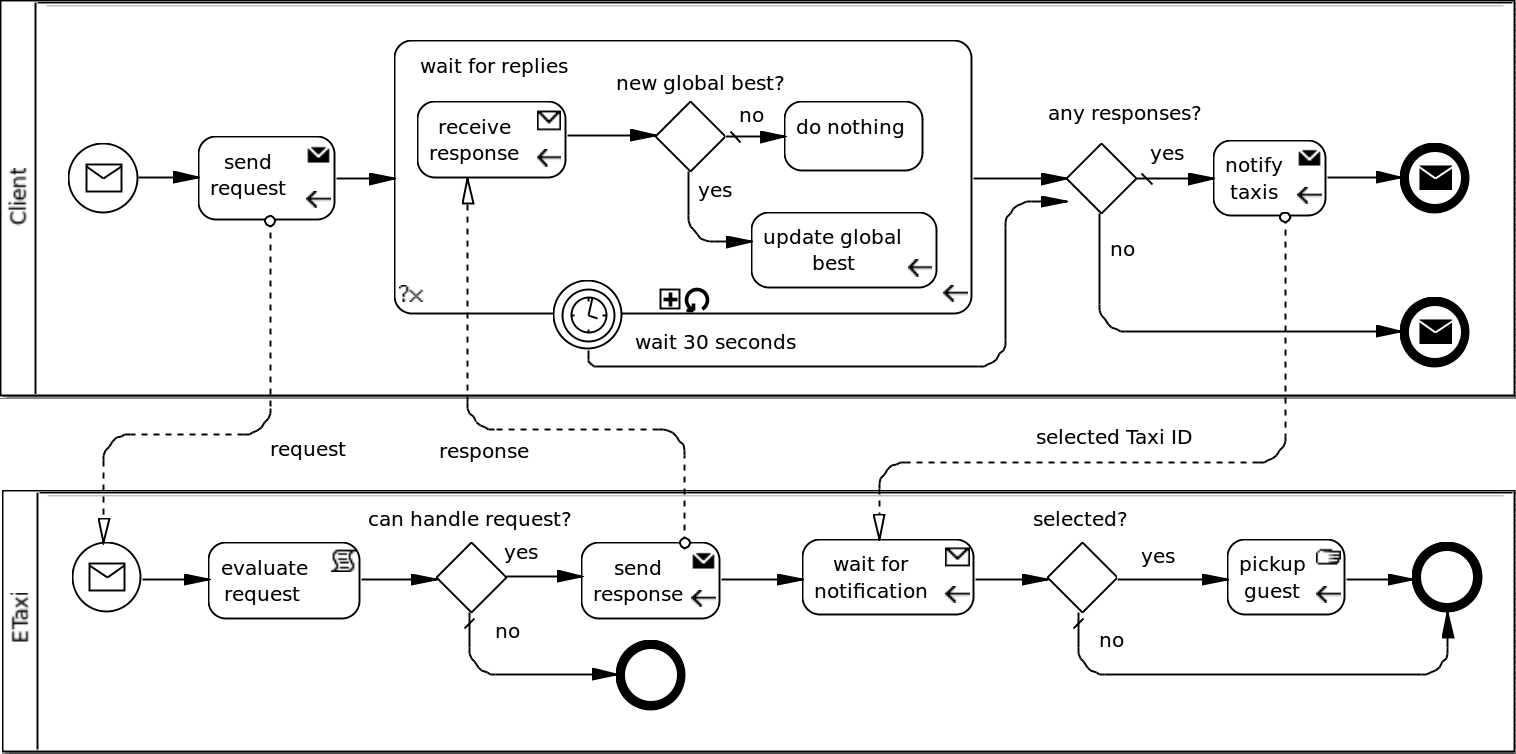
\includegraphics[width=\textwidth]{img/example.png}
	\caption{Example: Taxi Request Service}
	\label{fig:example}
\end{figure*}

% Beschreibung des Beispielprozesses
The BPMN diagram consists of two Pools, each representing an agent role: Client,
and E-Taxi.  The Client's process starts by broadcasting a request (customer ID,
location, destination, desired time of arrival) to all available E-Taxis, which
evaluate the request and decide whether they can handle it, in which case they
send a response (taxi ID, estimated time of arrival, price).  The Client enters
a looping subprocess, listening to responses and memorizing the best response,
until after 30 seconds the subprocess is interrupted by the attached timer event.
The Client then sends notifications to the responding E-Taxis, and the selected
E-Taxi prepares to pick up the guest.  Note that the several properties (variables)
and assignments are not visualized in the diagram.

% Sourcecode-Listing
The resulting Agent Bean for the Client role is shown in Listing~\ref{lst:example1},
slightly shortened to improve readability and to better fit into this paper.

\lstinputlisting[language=Java, caption=Generated Agent Bean: Client\_requestTaxi,
                 label=lst:example1]{img/example1.java}

% Beschreibung der Haupt-Klasse
As can be seen, the control-flow of the process is reflected in the workflow-method
\verb_requestTaxi()_, which is also exposed as a JIAC Action, or Service.  The
workflow-method is dominated by the threads for running the subprocess and the
attached event handler, but also contains an if-else-statement for the Gateway
at the end of the process.  The activities \emph{send request} and \emph{notify
taxis} are mapped to two similar methods for sending a JIAC message to the
specified broadcast message group.

% Beschreibung der inneren Klassen
The subprocess is mapped to an inner class, also forming a new variable scope for
the properties of the subprocess.  It features another workflow-method and several
activity-methods, most notably the \emph{receive responses} method, in which the
Client joins the specified message group and checks its memory for accordant
messages.  The subprocess is executed as a thread which is to be interrupted by
the event handler thread.  Both are shown in Listing~\ref{lst:example2}.

\lstinputlisting[language=Java, caption=Inner Classes for Subprocess and Event Handler,
                 label=lst:example2]{img/example2.java}


	%%%%%%%%%%%%%%%%%%%%%%%%%%%%%%%%%%%%%%%%%%%%%%%%%%%%%%%%%%%%%%%%%%%%%%%%%%%%%%%%
%%                                                                            %%
%%  CONCLUSION                                                                %%
%%                                                                            %%
%%%%%%%%%%%%%%%%%%%%%%%%%%%%%%%%%%%%%%%%%%%%%%%%%%%%%%%%%%%%%%%%%%%%%%%%%%%%%%%%

% [x] Zusammenfassung
% [x] Diskussion
% [x] Future Work

\section{Conclusion}
\label{sec:conclusion}

% kurze Zusammenfassung des Papers und des Mappings
In this paper, we have presented a new approach of creating multi-agent systems from
process models, combining the mapping from BPMN to JADL~\cite{kuester2010integrating}
with ideas borrowed from WADE~\cite{caire2008wade}.  The result is a transformation
from BPMN process diagrams to JIAC Agent Beans, comprising one method for the
workflow as a whole, and one method for each individual activity, but also
supporting beneficial aspects of BPMN such as messaging and event handling.


%%%%%%%%%%%%%%%%%%%%%%%%%%%%%%%%%%%%%%%%%%%%%%%%%%%%%%%%%%%%%%%%%%%%%%%%%%%%%%%%

\subsection{Discussion}

% alles ausdrückbar, was man modellieren kann
Using the domain-specific scripting language JADL, agent behaviours can be
expressed in a very compact and readable way, but the overall expressiveness is
limited.  JIAC Agent Beans, on the other hand, have the full expressiveness of
the Java language at their disposal.  Thus, basically everything that can be
modelled in a BPMN diagram can be mapped to an Agent Bean.

% etwas schwer verständlich, erweiterbar
While the resulting workflow-methods for complex processes can become somewhat
bulky -- particularly if event handlers are used -- the separation into
workflow-methods and activity-methods keeps the resulting code reasonably clear.
Further, like in WADE, individual activity-methods can be altered or extended
without risk of losing the changes after the code is generated anew.

% Schlusssatz: Wofür eignen sich die AgentBeans, und wofür die JADL-Services?
One drawback compared to the mapping to JADL scripts is that the generated Agent
Beans -- being Java classes -- can not as easily be deployed to an agent at runtime.
Regarding the high expressiveness of the generated Agent Beans and the good
performance of compiled Java code compared to the interpreted JADL scripts, the
mapping from BPMN to JIAC Agent Beans is suited best for modelling and generating
core components of the agents, while the mapping to JADL is of much use for
creating dynamic behaviours and services to be deployed and changed at runtime.


%%%%%%%%%%%%%%%%%%%%%%%%%%%%%%%%%%%%%%%%%%%%%%%%%%%%%%%%%%%%%%%%%%%%%%%%%%%%%%%%

\subsection{Future Work}

While the mapping can already be used for generating useful agent behaviours,
it is not yet completed.  First, there are still aspects of BPMN, which are not
covered by the mapping, such as some of the less common event types.  Second,
there are aspects of agents that can not yet be modelled adequately with BPMN.

Among the latter are messages to individual agents.  Originally, BPMN knew only
services and service calls.  In the course of our work, we extended our `dialect'
of BPMN with broadcast message groups, but what's still missing are messages to
individual agents, as identified by their agent ID.

Another issue which we want to tackle in the future is the modelling of goals by
means of BPMN.  One approach that appears to be promising is to use the
\emph{ad-hoc} subprocess for this task, but this is still work in progress.



	\bibliography{bibliography}

\end{document}

